\subsubsection{Use Cases} % (fold)
\label{ssub:usecasesold}

In the following tables the current supported use cases are explained step by step.
The first use case is detailed in Table~\ref{tab:usecasestopdevice}, explaining the situation where the user wants to stop/delete the session in a device.

\begin{center}
  \begin{usecase}[Stop a session of a device]
    \label{tab:usecasestopdevice}%
    \usecaseactor{System user}
    \usecasepre{A session is already running on a device, and it is showing in the \ida{PNAI} interface inside of that device.}
    \usecasepost{Session must terminate, i.e., the content must stop playing. The user must be notified with a popup and the session icon must be deleted from the \ida{PNAI} interface.}
    \usecasemain{
      \begin{usecasepath}
        \item User starts dragging the session icon.
        \item A copy of the session icon appears under the user's cursor, and follows the cursor until the user drops it.
        \item User drops the cloned session icon into the trash.
        \item A popup appears to notify the user that the action is in progress and the cloned session icon is deleted from the view.
        \item The content stops playing.
        \item The popup disappears and the original session icon is deleted from the view.
      \end{usecasepath}
    }
    \usecasealt{1}{
      \begin{usecasepath}[b]
        \setcounter{enumi}{2}
        \item User drops the session into a blank space.
        \item Action is cancelled.
      \end{usecasepath}
    }
    \usecasealt{2}{
      \begin{usecasepath}[c]
        \setcounter{enumi}{4}
        \item There is an error with the server and the content keeps playing.
        \item The content of the popup changes to notify the user that there was an error with the server and the action could not be completed.
        After 5 seconds it disappears.
        \item Action is cancelled.
      \end{usecasepath}
    }
  \end{usecase}
\end{center}

\begin{figure}[htbp]
  \centering
    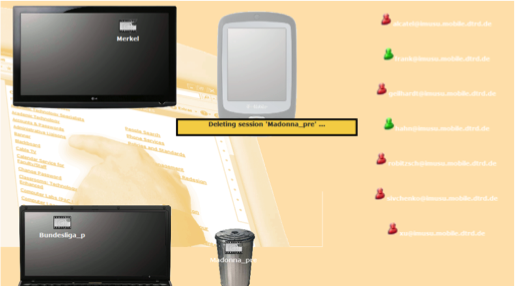
\includegraphics[width=\textwidth]{pnai-old-stop}
  \caption{Deleting a session in the old \idas{PNAI}}
  \label{fig:pnai-old-stop}
\end{figure}

Figure~\ref{fig:pnai-old-stop} shows how the page looks when it is waiting for a response to the server for the previous use case.
Since the user interface does not block in the process, the communication between the front end and the back end must be asynchronous.
The use case for terminating a session that a buddy is playing and that we own is very similar, as Table~\ref{tab:usecasestopbuddy} exposes.

\begin{center}
  \begin{usecase}[Stop a session of a buddy]
    \label{tab:usecasestopbuddy}%
    \usecaseactor{System user}
    \usecasepre{A session owned by the user is running on a device, and it is showing in the \ida{PNAI} interface near that buddy's name.}
    \usecasepost{Session must terminate, i.e., the content must stop playing. The user must be notified with a popup and the session icon must be deleted from the \ida{PNAI} interface. The buddy is \emph{not} notified, the content stops without warning.}
    \usecasemain{
      \begin{usecasepath}
        \item User starts dragging the session icon.
        \item A copy of the session icon appears under the user's cursor, and follows the cursor until the user drops it.
        \item User drops the cloned session icon into the trash.
        \item A popup appears to notify the user that the action is in progress and the cloned session icon is deleted from the view.
        \item The content stops playing.
        \item The popup disappears and the original session icon is deleted from the view.
      \end{usecasepath}
    }
    \usecasealt{1}{
      \begin{usecasepath}[b]
        \setcounter{enumi}{2}
        \item User drops the session into a blank space.
        \item Action is cancelled.
      \end{usecasepath}
    }
    \usecasealt{2}{
      \begin{usecasepath}[c]
        \setcounter{enumi}{4}
        \item There is an error with the server and the content keeps playing.
        \item The content of the popup changes to notify the user that there was an error with the server and the action could not be completed.
        After 5 seconds it disappears.
        \item Action is cancelled.
      \end{usecasepath}
    }
  \end{usecase}
\end{center}

Tables~\ref{tab:usecasecopydevice},~\ref{tab:usecasecopybuddy},~\ref{tab:usecasetransferdevice}~and~\ref{tab:usecasetransferbuddy} show how the user could copy or transfer a session to another device or buddy.

\begin{center}
  \begin{usecase}[Copy a session to a device]
    \label{tab:usecasecopydevice}%
    \usecaseactor{System user}
    \usecasepre{A session is already running on a device/buddy, and it is showing in the \ida{PNAI} interface inside of that device/buddy. Also, there is another device online.}
    \usecasepost{Session must be copied to that device, i.e., the content must be duplicated and played on that device. The user must be notified with a popup and the session icon must appear in the \ida{PNAI} interface for the second device.}
    \usecasemain{
      \begin{usecasepath}
        \item User starts dragging the session icon.
        \item A copy of the session icon appears under the user's cursor, and follows the cursor until the user drops it.
        \item User drops the cloned session icon into another device that is online.
        \item A popup menu appears where the user dropped the session, giving options to copy/duplicate the session, transfer the session or cancel the action.
        \item The user clicks on the copy/duplicate option.
        \item The popup menu disappears.
        \item A popup appears to notify the user that the action is in progress and the cloned session icon is deleted from the view.
        \item The content starts playing on the destination device.
        \item The popup disappears and the same session icon appears inside of the destination device.
      \end{usecasepath}
    }
    \usecasealt{1}{
      \begin{usecasepath}[b]
        \setcounter{enumi}{2}
        \item User drops the session into a blank space.
        \item Action is cancelled.
      \end{usecasepath}
    }
    \usecasealt{2}{
      \begin{usecasepath}[c]
        \setcounter{enumi}{4}
        \item The user clicks on the cancel option.
        \item Popup menu disappears and action is cancelled.
      \end{usecasepath}
    }
    \usecasealt{3}{
      \begin{usecasepath}[d]
        \setcounter{enumi}{7}
        \item There is an error with the server and the content is not duplicated.
        \item The content of the popup changes to notify the user that there was an error with the server and the action could not be completed.
        After 5 seconds it disappears.
        \item Action is cancelled.
      \end{usecasepath}
    }
  \end{usecase}
\end{center}

\begin{center}
  \begin{usecase}[Copy a session to a buddy]
    \label{tab:usecasecopybuddy}%
    \usecaseactor{System user}
    \usecasepre{A session is already running on a device/buddy, and it is showing in the \ida{PNAI} interface inside of that device/buddy. Also, there is another buddy online.}
    \usecasepost{Session must be copied to that buddy, i.e., the content must be duplicated and played on the buddy's default device. The user must be notified with a popup and the session icon must appear in the \ida{PNAI} interface near the name of that buddy. The buddy is \emph{not} notified, the content plays without warning.}
    \usecasemain{
      \begin{usecasepath}
        \item User starts dragging the session icon.
        \item A copy of the session icon appears under the user's cursor, and follows the cursor until the user drops it.
        \item User drops the cloned session icon into another buddy that is online.
        \item A popup menu appears where the user dropped the session, giving options to copy/duplicate the session, transfer the session or cancel the action.
        \item The user clicks on the copy/duplicate option.
        \item The popup menu disappears.
        \item A popup appears to notify the user that the action is in progress and the cloned session icon is deleted from the view.
        \item The content starts playing on the buddy's default device.
        \item The popup disappears and the same session icon appears inside of the destination buddy.
      \end{usecasepath}
    }
    \usecasealt{1}{
      \begin{usecasepath}[b]
        \setcounter{enumi}{2}
        \item User drops the session into a blank space.
        \item Action is cancelled.
      \end{usecasepath}
    }
    \usecasealt{2}{
      \begin{usecasepath}[c]
        \setcounter{enumi}{4}
        \item The user clicks on the cancel option.
        \item Popup menu disappears and action is cancelled.
      \end{usecasepath}
    }
    \usecasealt{3}{
      \begin{usecasepath}[d]
        \setcounter{enumi}{7}
        \item There is an error with the server and the content is not duplicated.
        \item The content of the popup changes to notify the user that there was an error with the server and the action could not be completed.
        After 5 seconds it disappears.
        \item Action is cancelled.
      \end{usecasepath}
    }
  \end{usecase}
\end{center}

\begin{center}
  \begin{usecase}[Transfer a session to a device]
    \label{tab:usecasetransferdevice}%
    \usecaseactor{System user}
    \usecasepre{A session is already running on a device/buddy, and it is showing in the \ida{PNAI} interface inside of that device/buddy. Also, there is another device online.}
    \usecasepost{Session must be transferred to that device, i.e., playback must be stopped at the source and started at the destination device. The user must be notified with a popup and the session icon must appear in the \ida{PNAI} interface for the second device.}
    \usecasemain{
      \begin{usecasepath}
        \item User starts dragging the session icon.
        \item A copy of the session icon appears under the user's cursor, and follows the cursor until the user drops it.
        \item User drops the cloned session icon into another device that is online.
        \item A popup menu appears where the user dropped the session, giving options to copy the session, transfer/hand over the session or cancel the action.
        \item The user clicks on the transfer/hand over option.
        \item The popup menu disappears.
        \item A popup appears to notify the user that the action is in progress and the cloned session icon is deleted from the view.
        \item The content stops playing on the source device.
        \item The content starts playing on the destination device.
        \item The popup disappears, the session icon is deleted from the view and created again inside of the destination device.
      \end{usecasepath}
    }
    \usecasealt{1}{
      \begin{usecasepath}[b]
        \setcounter{enumi}{2}
        \item User drops the session into a blank space.
        \item Action is cancelled.
      \end{usecasepath}
    }
    \usecasealt{2}{
      \begin{usecasepath}[c]
        \setcounter{enumi}{4}
        \item The user clicks on the cancel option.
        \item Popup menu disappears and action is cancelled.
      \end{usecasepath}
    }
    \usecasealt{3}{
      \begin{usecasepath}[d]
        \setcounter{enumi}{7}
        \item There is an error with the server and the content is not transferred.
        \item The content of the popup changes to notify the user that there was an error with the server and the action could not be completed.
        After 5 seconds it disappears.
        \item Action is cancelled.
      \end{usecasepath}
    }
  \end{usecase}
\end{center}

\begin{center}
  \begin{usecase}[Transfer a session to a buddy]
    \label{tab:usecasetransferbuddy}%
    \usecaseactor{System user}
    \usecasepre{A session is already running on a device/buddy, and it is showing in the \ida{PNAI} interface inside of that device/buddy. Also, there is another buddy online.}
    \usecasepost{Session must be transferred to that buddy, i.e., playback must be stopped at the source and started at the buddy's default device. The user must be notified with a popup and the session icon must appear in the \ida{PNAI} interface near the name of that buddy. The buddy is \emph{not} notified, the content plays without warning.}
    \usecasemain{
      \begin{usecasepath}
        \item User starts dragging the session icon.
        \item A copy of the session icon appears under the user's cursor, and follows the cursor until the user drops it.
        \item User drops the cloned session icon into another buddy that is online.
        \item A popup menu appears where the user dropped the session, giving options to copy the session, transfer/hand over the session or cancel the action.
        \item The user clicks on the transfer/hand over option.
        \item The popup menu disappears.
        \item A popup appears to notify the user that the action is in progress and the cloned session icon is deleted from the view.
        \item The content stops playing on the source device.
        \item The content starts playing on the buddy's default device.
        \item The popup disappears, the session icon is deleted from the view and created again inside of the destination buddy.
      \end{usecasepath}
    }
    \usecasealt{1}{
      \begin{usecasepath}[b]
        \setcounter{enumi}{2}
        \item User drops the session into a blank space.
        \item Action is cancelled.
      \end{usecasepath}
    }
    \usecasealt{2}{
      \begin{usecasepath}[c]
        \setcounter{enumi}{4}
        \item The user clicks on the cancel option.
        \item Popup menu disappears and action is cancelled.
      \end{usecasepath}
    }
    \usecasealt{3}{
      \begin{usecasepath}[d]
        \setcounter{enumi}{7}
        \item There is an error with the server and the content is not transferred.
        \item The content of the popup changes to notify the user that there was an error with the server and the action could not be completed.
        After 5 seconds it disappears.
        \item Action is cancelled.
      \end{usecasepath}
    }
  \end{usecase}
\end{center}

\begin{figure}[htbp]
  \centering
    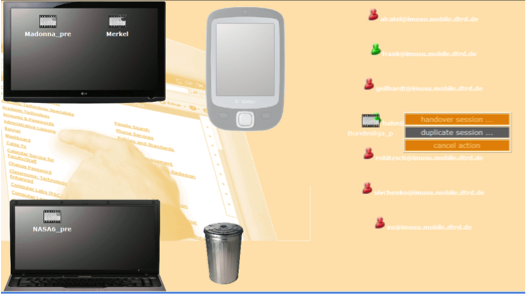
\includegraphics[width=\textwidth]{pnai-old-duplicate}
  \caption{Duplicating a session in the old \idas{PNAI}}
  \label{fig:pnai-old-duplicate}
\end{figure}

Figure~\ref{fig:pnai-old-duplicate} shows how the popup menu is displayed to the user.
It is a very simple menu with only three links, each of which correspond to an action.
% subsubsection usecasesold (end)